\chapter{O Tema da Tese}

\begin{center}
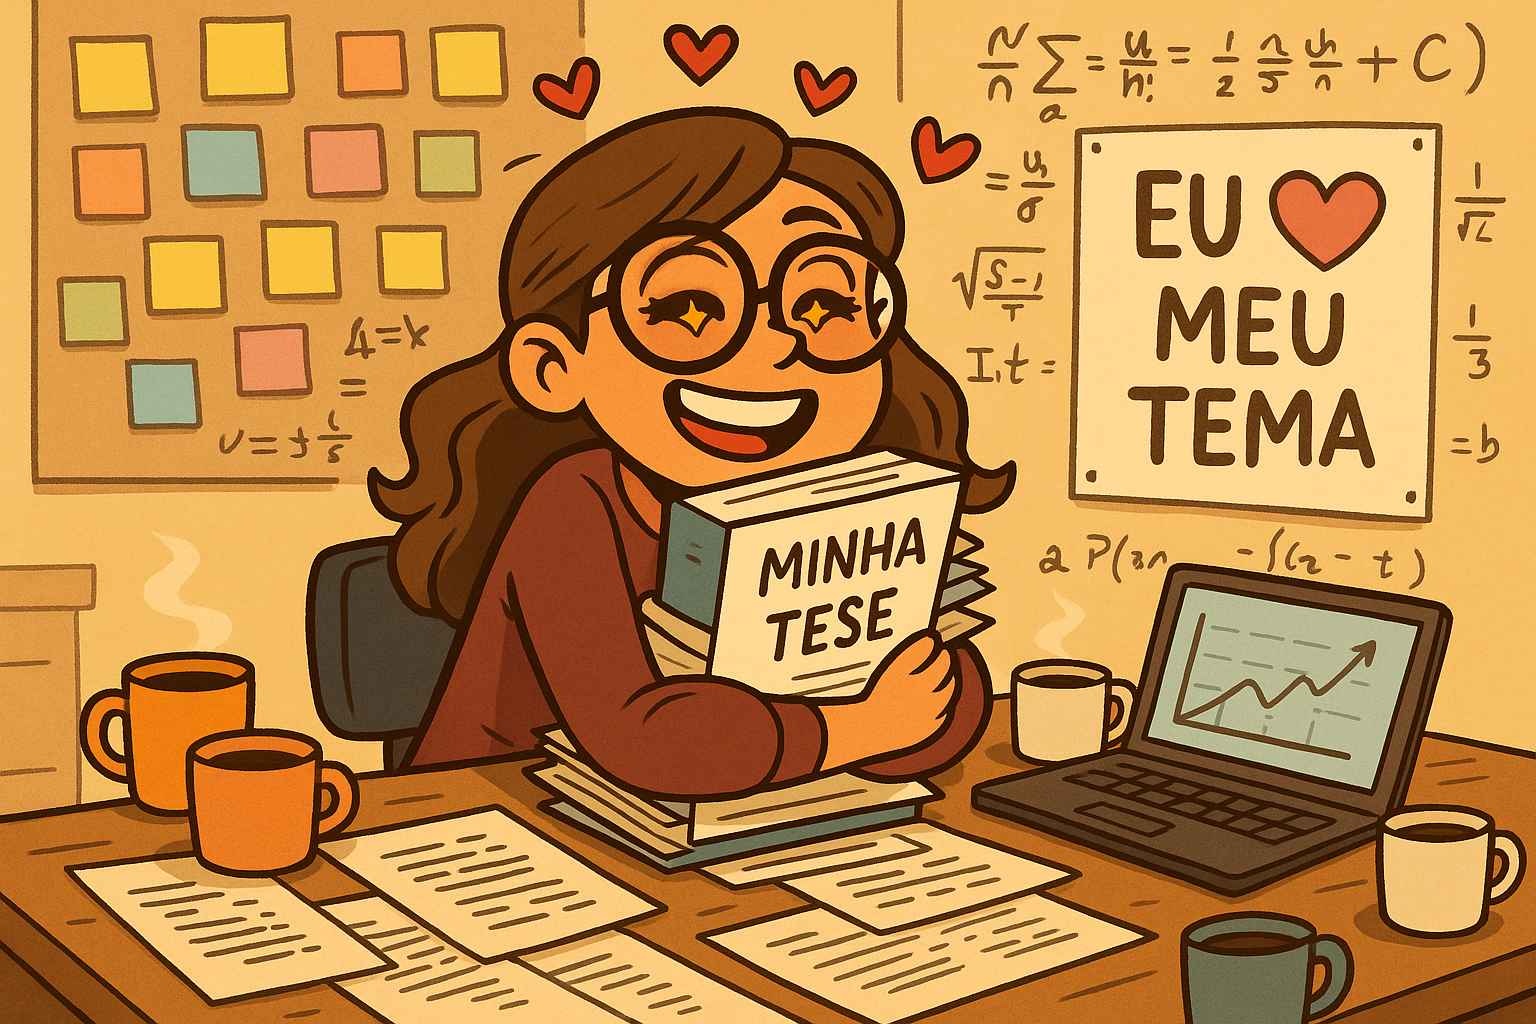
\includegraphics[width=0.5\linewidth]{Images/amomeutema.png}    
\end{center}
\vspace{0.5cm}

A tese obrigatoriamente tem que ter um assunto, que deve ser escolhido no início do trabalho. Essa escolha é importante e deve ser feita com cuidado, de modo a que permita ao candidato crescer academicamente, contribuir para o conhecimento e, ao mesmo tempo, evitar dissabores.

\gxatencao{O aluno deve se identificar fortemente \\ com o tema de tese escolhido.}

Você não vai conseguir acabar uma tese da qual não goste do tema desde o início do seu trabalho. Mesmo gostando do tema inicialmente, é possível que no fim da tese você não queira ver mais o tema ``nem pintado'', o que não é bom, mas pelo menos você terminou a tese.

O tema deve ser escolhido com muito cuidado. Primeiro, deve ser de seu interesse, praticamente uma paixão. Segundo, deve ser de interesse do orientador. Finalmente, deve ser do interesse da comunidade científica.

Alguns temas, mesmo sendo de interesse pessoal, não interessam a ninguém. Ou por já estarem resolvidos, ou por não serem ainda percebidos, ou pior, porque não têm valor científico, ou não têm valor na comunidade científica a que o candidato pertence.

Normalmente se faz um plano de tese no início. Esse plano nem sempre é seguido, pois com o tempo entendemos melhor o problema, suas formas mais genéricas ou mais específicas, e alterações de rota são feitas.

Não se preocupe muito no início, no primeiro ano do doutorado, ou nos três primeiros meses de pesquisa no mestrado, se seu tema é incerto. Seu objetivo deve ser fixado nesse prazo, mas o mais importante é entender o contexto do tema e os problemas importantes a serem resolvidos. Depois, nos próximos 2 ou 3 anos, você irá em direção a fechar a tese.

Para escolher o tema, é importante que você escolha cadeiras que tenham relação com assuntos de seu interesse. Não escolha cadeiras pela facilidade ou pelo horário disponível, escolha cadeiras que lhe ajudem a escolher e estudar temas de seu interesse.

% TODO: \usepackage{graphicx} required
\begin{figure}[hbt]
    \centering
    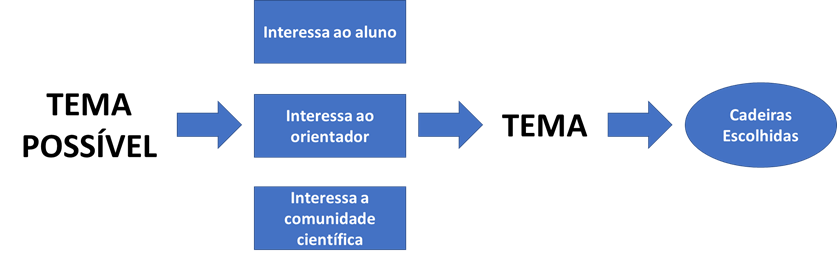
\includegraphics[width=0.9\linewidth]{Images/escolhatemacadeiras}
    \caption{Escolhendo tema e cadeiras. Fonte: o autor}
    \label{fig:escolhatemacadeiras}
\end{figure}


\section{O que é uma Contribuição Original}

Um dos requisitos da tese de doutorado é possuir uma contribuição original.

Eu confesso que contribuição original não é uma definição muito clara. Vamos analisar, então, o que é uma contribuição.

A professora Marta Mattoso diz que :
\begin{itemize}
\item	“Uma contribuição é um resultado que pode ser útil para outras pessoas.”
\item	“O resultado é uma novidade e não poderia ser afirmado sem o desenvolvimento da tese.”
\end{itemize}

Ou seja, uma contribuição pode se algo como encontrado na lista a seguir, levemente ordenada da maior para a menor e de forma não exaustiva.
\begin{enumerate}
\item	A solução de um problema em aberto;
\item	Uma melhoria comprovada a alguma prática da área;
\item	A proposta de uma metodologia, método ou processo que resolva um problema do mundo real, com uma abordagem científica;
\item	Aplicar uma prática da área em uma área de aplicação, de maneira não trivial;
\item	A investigação de um problema que descobre novas evidências na área;
\item	A criação de sistemas complexos envolvendo várias práticas até antes isoladas, com um resultado científico palpável;
\item	A comparação e análise de diferentes soluções computacionais para o mesmo problema, com consequente desenvolvimento de solução que as agregam de alguma forma;
\item	O levantamento de uma história, ou o estudo de casos, que trazem contribuição original para o entendimento de como algo aconteceu ou acontece, sempre de acordo com metodologias reconhecidas;
\item	A criação de novas bases de dados que podem servir para outros trabalhos.
\end{enumerate}


Veja que a tese tem que comprovar a contribuição. Não basta dizer que algo é bom e original, é importante poder provar que é melhor (mesmo que dentro de alguns casos) e que não há outro resultado igual, ou ainda que abre um caminho novo de pesquisa.

\CoppeWay{O que não é contribuição}{
Porém, ao contrário de outras áreas, no Programa de Engenharia de Sistemas e Computação, e em toda Coppe, não é considerada uma contribuição;
\begin{itemize}
    \item 	Fazer a compilação de dados ou informações já existentes (como a criação de um review da área);
    \item	Desenvolver aplicações convencionais com software disponível amplamente;
    \item 	Desenvolver protótipos de aplicações semelhantes a outras e com tecnologia amplamente conhecida e divulgada.
\end{itemize}
}

\section{Como encontrar uma Contribuição}

Normalmente em uma tese de Computação existe um problema, uma solução e uma comprovação ou validação da solução. 

Assim, uma tese pode apresentar contribuições nessas três áreas. Lidando com o problema, podemos encontrar novos problemas ainda não tratados e modelar de formas diferentes problemas já tratados.

Na solução, podemos aplicar técnicas já existentes em problemas ainda não tratados com elas ou inventar novas técnicas. Finalmente, podemos trabalhar arduamente nas técnicas de comprovação de nossos resultados, principalmente quando esses resultados são experimentais ou empíricos\footnote{Em soluções teóricas é necessário provar que a solução é verdadeira, porém isso normalmente é parte da própria solução. Porém, existem teses teóricas que apresentam novas formas, mais simples, de provar um teorema já provado}.

O importante é ter um problema bem claro. Esse problema pode já ter sido proposto antes, ou pode ser levantado. Uma maneira de levantar problemas é estudar soluções já existentes e ver quando elas falham, ou que lacunas elas têm. 

Listar as falhas ou lacunas de uma situação atual é um bom método de descobrir onde você pode trabalhar. As lacunas podem ser elencadas, algumas podem ser selecionadas, e toda a tese construída em torno desse conceito.

O problema é o porquê de sua tese. Sua motivação. Não há como entender o que fazer se não é entendido primeiro por que aquilo é necessário, já que os requisitos de sua solução são definidos pelas necessidades do problema. Esses requisitos vão definir como sua proposta de solução será avaliada no final.

Muitos alunos querem começar pela solução, algo do tipo “quero usar a técnica X”. Esse não é um bom caminho, apesar de já ter funcionado para algumas pessoas. Porém, o que acontece normalmente é que o aluno fica com uma solução à procura de um problema e não tem como comprovar a qualidade ou a utilidade de sua solução.


\section{Pensando sua Tese}

Várias técnicas podem ser usadas para você pensar sua tese.
Para começar, quando achar que algo é um bom tema:
\begin{itemize}
    \item Escreva uma sentença de até 25 palavras sobre o tema da sua tese.
    \item Não misture mais de 2 áreas de pesquisa.
    \item Encontre primeiro o problema, depois a solução.
\end{itemize}

 Uma das técnicas mais gerais e mais úteis é \gxdefine{5W2H}, responder as perguntas: Why, What, Who, When, Where, How e How Much. 
Principalmente se perguntar “Por que estou fazendo isso” e “Quem vai ser beneficiado” permite justificar plenamente o trabalho de sua tese, fazendo com que ela não fique perdida em um contexto vago. 
A Figura \ref{fig:5w2h} mostra algumas perguntas possíveis nessa técnica.

% TODO: \usepackage{graphicx} required
\begin{figure}[hbt]
    \centering
    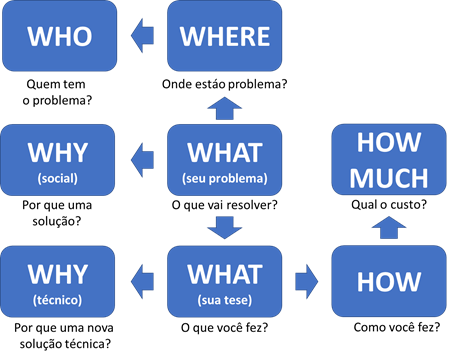
\includegraphics[width=0.7\linewidth]{Images/5w2h}
    \caption{Perguntas que devem ser respondidas antes de iniciar uma tese. Fonte: do autor.}
    \label{fig:5w2h}
\end{figure}

AS teses, muitas vezes, investigam lacunas específicas no estado da arte, por exemplo, buscando em trabalhos futuros, ou buscando problemas reconhecidamente não resolvidos ou onde o estado da arte ainda não é considerado uma solução eficiente ou eficaz. 
A partir dessas lacunas podem ser geradas questões de pesquisa, que por sua vez podem gerar objetivos gerais e específicos. Esse é um bom quadro teórico para trabalhar.

Essa busca de lacunas também pode ser feita com pesquisas e entrevistas, onde por meio de métodos como a \gxdefine{Análise de Conteúdo}\citep{bardin2011analise} ou a \textit{Grounded Theory}\citep{glaser1967discovery}, se desenvolve uma teoria onde algo precisa ainda ser feito. O próprio desenvolvimento dessa teoria, i.e., o modelo, pode ser um tema de tese.

Entre meus alunos, o uso da \gxdefine{Design Science Research} (\gxdefine{DSR})\citep{pimentel2023} também fornece caminhos para pensar sua tese . Eu estou me tornando cada vez mais um adepto dessa abordagem, 
que se configura não como um método único, mas como uma filosofia de pesquisa  
capaz de abrigar diferentes processos metodológicos mais específicos\citep{hevner2004design,Dresch2014,march1995design,pimentel2023}.

Em síntese, a DSR propõe que o pesquisador proponha um artefato que resolve um problema em um contexto, e o avalie de forma correta\citep{pimentel2023}.  
Dessa forma, o pesquisador mantém um ciclo iterativo de construção e validação que alinha relevância prática e contribuição científica. Na Seção \ref{sec:dsr} ela é discutida um pouco mais profundamente.

\section{Project Model Canvas}

Outra técnica possível, e complementar a todas as outras, é desenhar um \gxdefine{Project Model Canvas}\footnote{\expurl{http://www.projectmodelcanvas.com/}{Project Model Canvas}} . Essa é uma proposta de José Finocchio Júnior e tem uma representação visual interessante, apresentada na Figura \ref{fig:pmc}. Realmente, uma tese é um projeto, porém não pode ser vista como um projeto igual o da indústria. Então, ao responder as perguntas implícitas no Canvas, é necessário levar em consideração a necessidade de fazer Ciência e não apenas de entregar um produto.

% TODO: \usepackage{graphicx} required
\begin{figure}
    \centering
    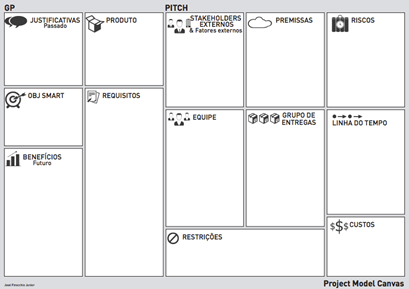
\includegraphics[width=0.7\linewidth]{Images/PMC}
    \caption{Representação do Project Model Canvas de José Finocchio Júnior (CC:BYNOND)}
    \label{fig:pmc}
\end{figure}


\section{Como descrever o que é a tese}

Algumas coisas são importantes para você definir sua tese.

Primeiro, você tem que \textbf{conhecer um problema} e o \textbf{estado da arte da solução} do problema. Se seu orientador trabalha com o problema, você ainda tem que conhecer bem o trabalho que ele tem feito, para entrar realmente no grupo.

Segundo, é interessante que você consiga dar um \textbf{valor} a esse problema\footnote{Você pode ouvir uma aula sobre valor em \expurl{https://youtu.be/aOQQHGzC-YE}{Aula introdutória em vídeo sobre valor}, ou ler o capítulo sobre valor escrito em \url{https://github.com/xexeo/MaterialEducacional}} . O valor pode ser econômico, como a diminuição de um custo, pode ser um valor acadêmico, como um teorema em aberto há muito tempo, ou pode ser outra forma de valor, como social ou histórico. Uma visão rápida de Valor, típica da Engenharia de Software, é procurar 3 coisas: aumentar o faturamento (benefícios), reduzir custos e melhorar serviços. Vale a pena também entender as formas de capital propostas por \citet{bourdieu1986forms}: o capital econômico, o capital cultural, o capital social e o capital simbólico. Como você cria um desses tipos de capital?

Terceiro, você deve ter uma \textbf{proposta de abordagem ao problema}. Isto significa que você deve entender caminhos possíveis para resolvê-lo e ter uma ideia das técnicas que pretende adotar.

Todas essas coisas podem ser descritas de várias formas, tanto ao longo do trabalho, em apresentações, como no texto final. Algumas abordagens são mais tradicionais do que outras.

\section{Uma Introdução da Tese que Evolui}

Uma prática interessante é manter uma introdução atualizada da tese ao longo do trabalho. 

Na introdução da sua tese deve existir uma descrição do que ela é e que deixe o leitor totalmente ciente do que vai encontrar durante a leitura. 

Como vimos, é importante \textbf{definir o problema} que a tese trata. Esse problema deve ocorrer dentro de um \textbf{contexto}. Também deve ficar claro o \textbf{objetivo} da tese. Esse objetivo pode ser dividido em \textbf{questões de pesquisa}, que devem levar gradativamente ao objetivo, ou pode gerar \textbf{conjecturas} que precisam ser comprovadas ou, pelo menos, validadas, já que certas conjecturas são difíceis de serem comprovadas de forma absoluta, devido a incluírem, por exemplo, aspectos do comportamento humano.

Costumamos reservar o termo \textbf{hipótese para conjecturas que podem ser provadas com experimentos} que inclui uma hipótese nula, por meios estatísticos, ou provada, ou negada, por meio de um teorema.
Cuidado porque algumas pessoas confundem o termo \textbf{premissa} com o termo hipótese. Tanto premissas como hipóteses podem ser suposições, porém as premissas são afirmações ou situações que consideramos verdadeiras, ou mesmo limitam o nosso escopo, enquanto hipóteses serão investigadas no trabalho.
Chamar de hipótese, no corpo da tese, algo que não pode ser comprovado experimental ou empiricamente, cria uma expectativa errada no leitor. 
Caso não haja uma comprovação formal, devemos evitar o termo hipótese e usar outros como conjecturas ou questões de pesquisa.

Sobre as premissas, elas podem também ser necessárias. Isso acontece quando o problema ou o contexto ainda são muito amplos em possibilidades, e é preciso considerar algumas coisas como verdade para poder começar a trabalhar. Premissas não são questionadas ao longo da tese, e sim assumidas como válidas. Claro que se espera que as premissas tenham alguma evidência, ou seja, não sejam facilmente falseáveis.


